\begin{frame}[allowframebreaks]{Vision Transformers (ViTs) Architecture}
    \textbf{Tokenizing Images:}
    \begin{itemize}
        \item \textbf{Input:} An image of size $H \times W \times C$ is divided into non-overlapping patches of size $P \times P$.
        \item Each patch is flattened into a vector and projected linearly to form patch embeddings.
        \item Positional encodings are added to retain spatial information.
    \end{itemize}

    \framebreak

    \begin{figure}
        \centering
        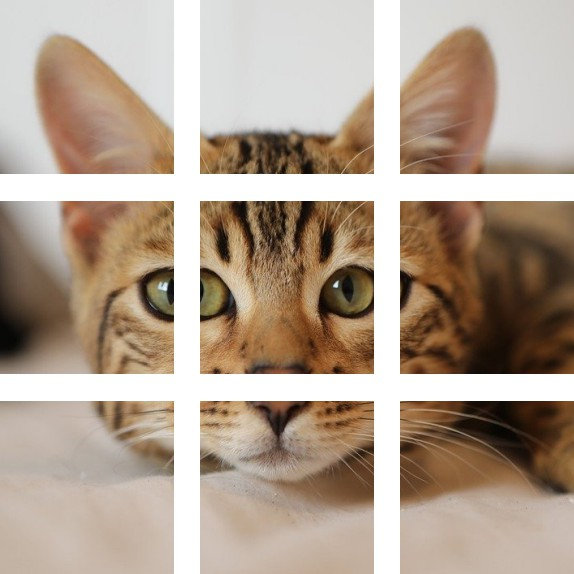
\includegraphics[width=\linewidth,height=0.9\textheight,keepaspectratio]{images/vit/slide_58_1_img.jpg}
    \end{figure}

    \framebreak

    \begin{figure}
        \flushleft
        
\includegraphics[width=0.85\linewidth,height=\textheight,keepaspectratio]{images/vit/slide_59_1_img.jpg}
    \end{figure}

    \framebreak

    \begin{figure}
        \flushleft
        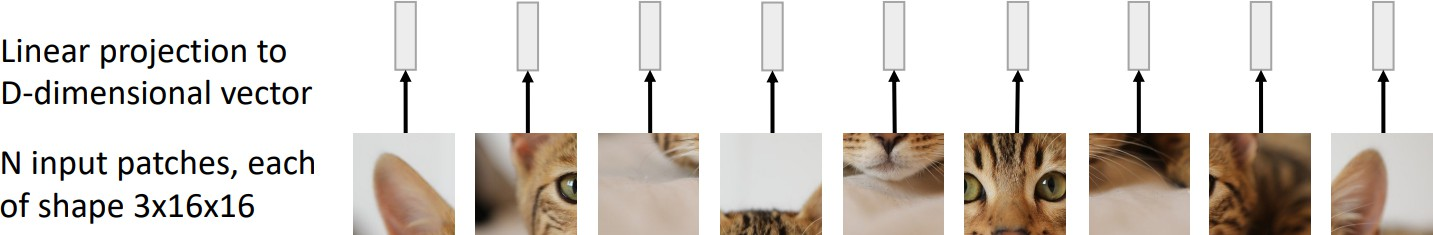
\includegraphics[width=0.85\linewidth,height=\textheight,keepaspectratio]{images/vit/slide_60_1_img.jpg}
    \end{figure}

    \framebreak

    \textbf{Transformer Encoder:}
    \begin{itemize}
        \item The sequence of patch embeddings, along with a special [CLS] token, is processed by standard Transformer encoder blocks.
        \item Each block consists of multi-head self-attention and feed-forward layers.
    \end{itemize}

    \framebreak

    \begin{figure}
        \flushleft
        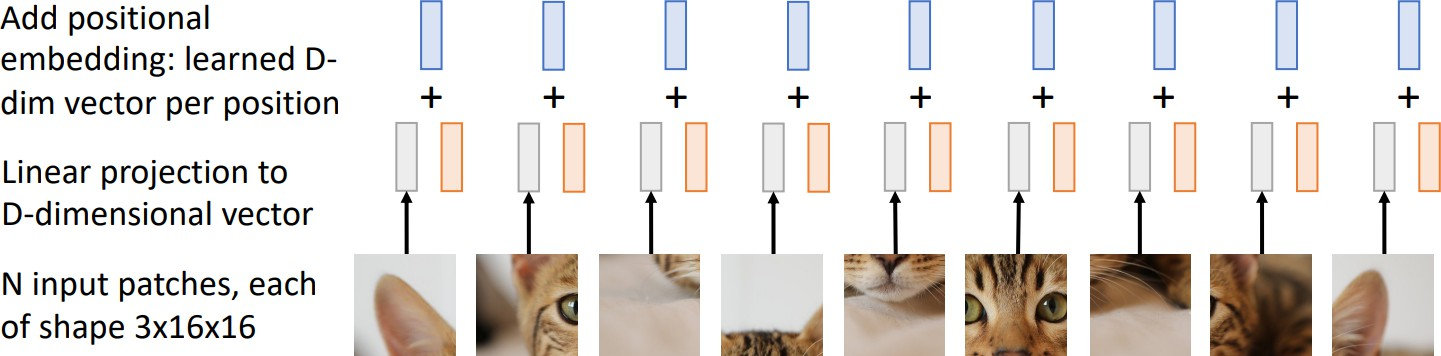
\includegraphics[width=0.85\linewidth,height=\textheight,keepaspectratio]{images/vit/slide_61_1_img.jpg}
    \end{figure}

    \framebreak

    \begin{figure}
        \flushleft
        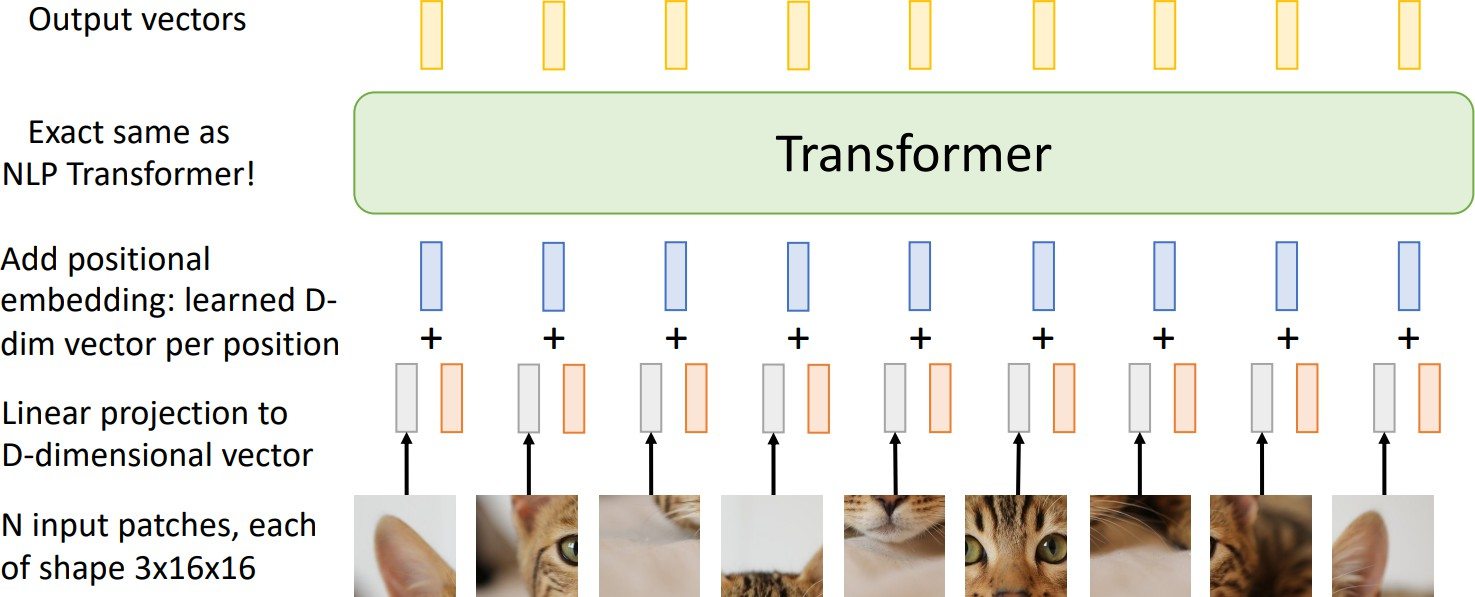
\includegraphics[width=0.85\linewidth,height=\textheight,keepaspectratio]{images/vit/slide_62_1_img.jpg}
    \end{figure}

    \framebreak

    \begin{figure}
        \flushleft
        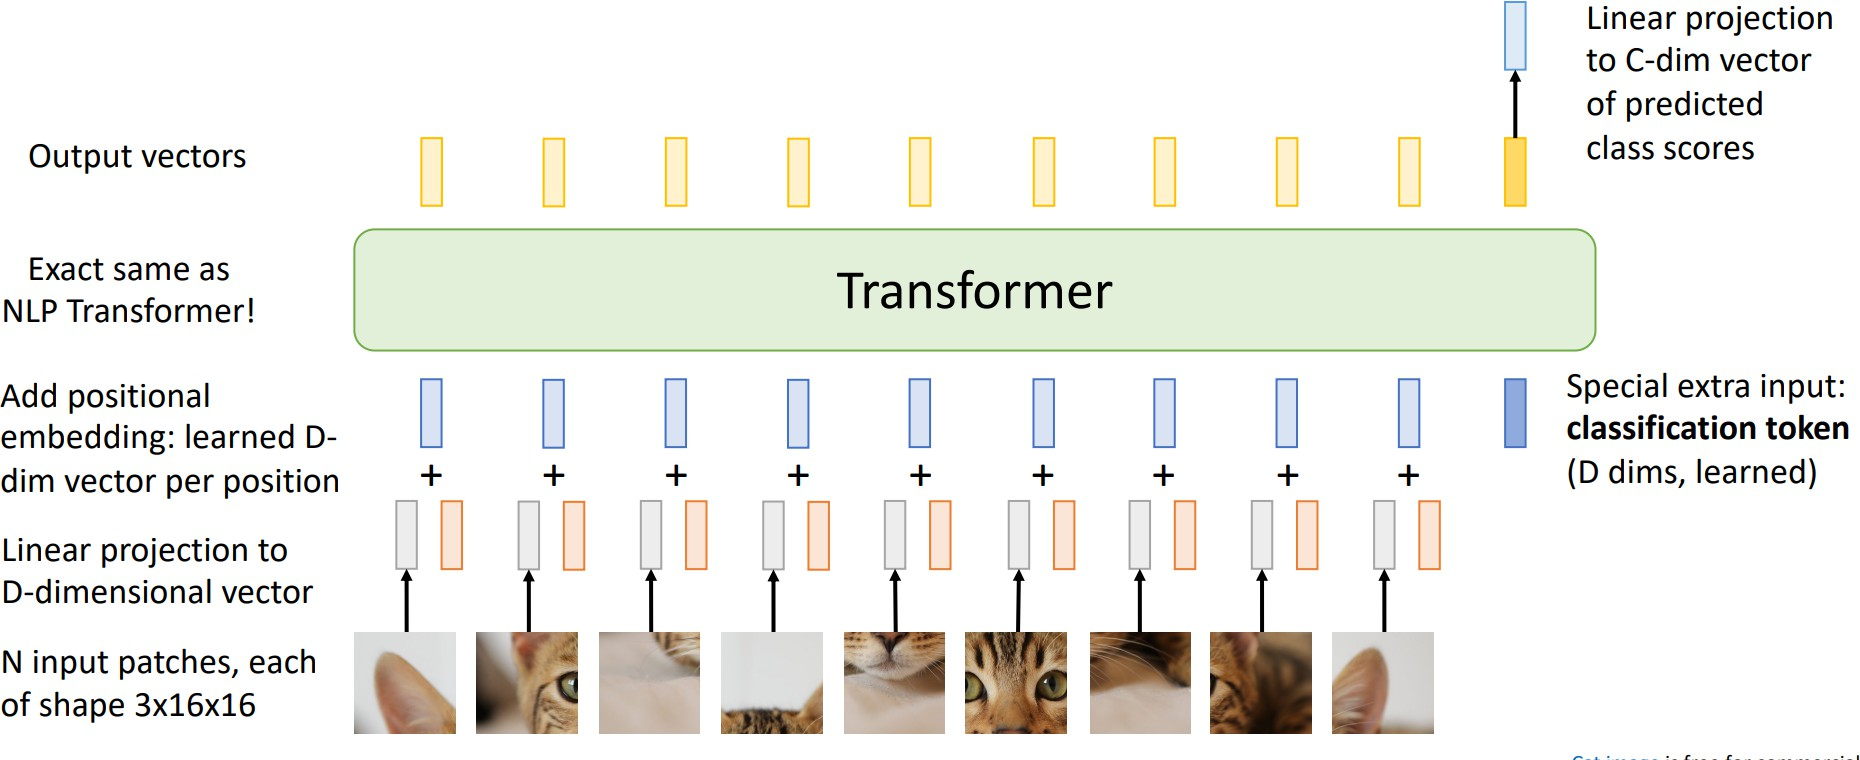
\includegraphics[width=\linewidth,height=\textheight,keepaspectratio]{images/vit/slide_63_1_img.jpg}
    \end{figure}

    \framebreak

    \textbf{Classification:}
    \begin{itemize}
        \item The output corresponding to the [CLS] token is used for image classification.
    \end{itemize}
    \vspace{1em}

    \textbf{Results:}
    \begin{itemize}
        \item ViT achieves competitive, often state-of-the-art, performance (e.g., 88--89\% top-1 accuracy on ImageNet) when trained on large datasets.
    \end{itemize}

    \framebreak

    \begin{figure}
        \flushleft
        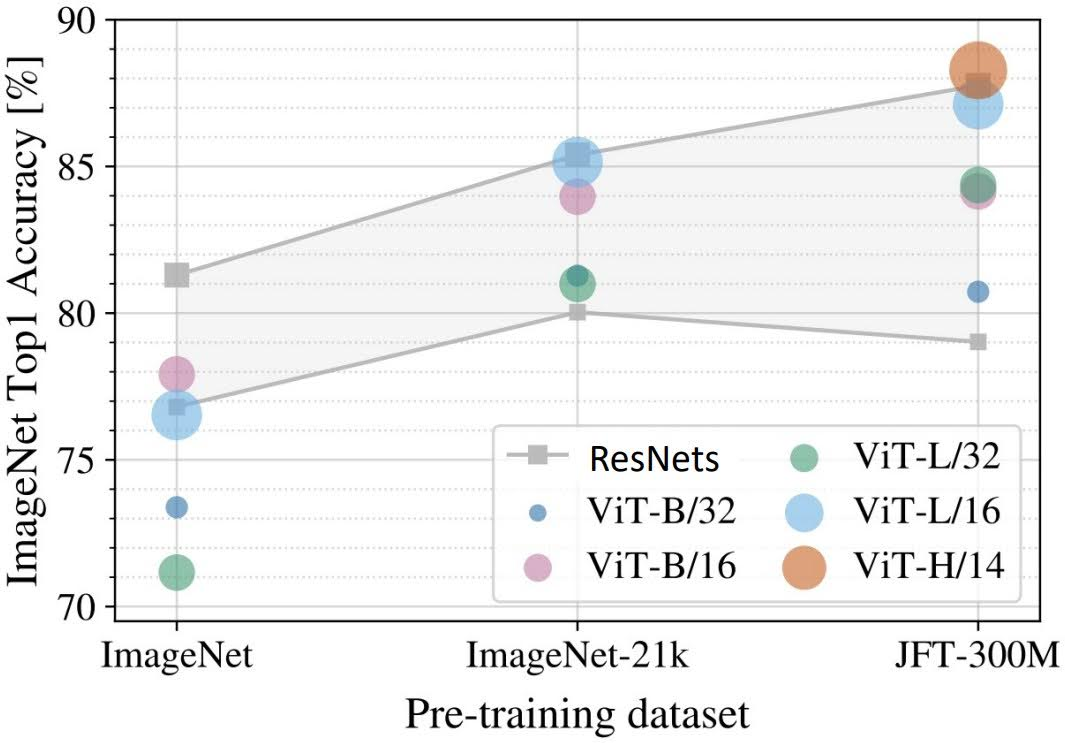
\includegraphics[width=\linewidth,height=0.8\textheight,keepaspectratio]{images/vit/slide_64_1_img.png}
        \footnote{Dosovitskiy et al, “An Image is Worth 16x16 Words: Transformers for Image Recognition at Scale”, ICLR 2021}
    \end{figure}
\end{frame}
